% Options for packages loaded elsewhere
\PassOptionsToPackage{unicode}{hyperref}
\PassOptionsToPackage{hyphens}{url}
%
\documentclass[
]{article}
\usepackage{amsmath,amssymb}
\usepackage{lmodern}
\usepackage{iftex}
\ifPDFTeX
  \usepackage[T1]{fontenc}
  \usepackage[utf8]{inputenc}
  \usepackage{textcomp} % provide euro and other symbols
\else % if luatex or xetex
  \usepackage{unicode-math}
  \defaultfontfeatures{Scale=MatchLowercase}
  \defaultfontfeatures[\rmfamily]{Ligatures=TeX,Scale=1}
\fi
% Use upquote if available, for straight quotes in verbatim environments
\IfFileExists{upquote.sty}{\usepackage{upquote}}{}
\IfFileExists{microtype.sty}{% use microtype if available
  \usepackage[]{microtype}
  \UseMicrotypeSet[protrusion]{basicmath} % disable protrusion for tt fonts
}{}
\makeatletter
\@ifundefined{KOMAClassName}{% if non-KOMA class
  \IfFileExists{parskip.sty}{%
    \usepackage{parskip}
  }{% else
    \setlength{\parindent}{0pt}
    \setlength{\parskip}{6pt plus 2pt minus 1pt}}
}{% if KOMA class
  \KOMAoptions{parskip=half}}
\makeatother
\usepackage{xcolor}
\usepackage[margin=1in]{geometry}
\usepackage{color}
\usepackage{fancyvrb}
\newcommand{\VerbBar}{|}
\newcommand{\VERB}{\Verb[commandchars=\\\{\}]}
\DefineVerbatimEnvironment{Highlighting}{Verbatim}{commandchars=\\\{\}}
% Add ',fontsize=\small' for more characters per line
\usepackage{framed}
\definecolor{shadecolor}{RGB}{248,248,248}
\newenvironment{Shaded}{\begin{snugshade}}{\end{snugshade}}
\newcommand{\AlertTok}[1]{\textcolor[rgb]{0.94,0.16,0.16}{#1}}
\newcommand{\AnnotationTok}[1]{\textcolor[rgb]{0.56,0.35,0.01}{\textbf{\textit{#1}}}}
\newcommand{\AttributeTok}[1]{\textcolor[rgb]{0.77,0.63,0.00}{#1}}
\newcommand{\BaseNTok}[1]{\textcolor[rgb]{0.00,0.00,0.81}{#1}}
\newcommand{\BuiltInTok}[1]{#1}
\newcommand{\CharTok}[1]{\textcolor[rgb]{0.31,0.60,0.02}{#1}}
\newcommand{\CommentTok}[1]{\textcolor[rgb]{0.56,0.35,0.01}{\textit{#1}}}
\newcommand{\CommentVarTok}[1]{\textcolor[rgb]{0.56,0.35,0.01}{\textbf{\textit{#1}}}}
\newcommand{\ConstantTok}[1]{\textcolor[rgb]{0.00,0.00,0.00}{#1}}
\newcommand{\ControlFlowTok}[1]{\textcolor[rgb]{0.13,0.29,0.53}{\textbf{#1}}}
\newcommand{\DataTypeTok}[1]{\textcolor[rgb]{0.13,0.29,0.53}{#1}}
\newcommand{\DecValTok}[1]{\textcolor[rgb]{0.00,0.00,0.81}{#1}}
\newcommand{\DocumentationTok}[1]{\textcolor[rgb]{0.56,0.35,0.01}{\textbf{\textit{#1}}}}
\newcommand{\ErrorTok}[1]{\textcolor[rgb]{0.64,0.00,0.00}{\textbf{#1}}}
\newcommand{\ExtensionTok}[1]{#1}
\newcommand{\FloatTok}[1]{\textcolor[rgb]{0.00,0.00,0.81}{#1}}
\newcommand{\FunctionTok}[1]{\textcolor[rgb]{0.00,0.00,0.00}{#1}}
\newcommand{\ImportTok}[1]{#1}
\newcommand{\InformationTok}[1]{\textcolor[rgb]{0.56,0.35,0.01}{\textbf{\textit{#1}}}}
\newcommand{\KeywordTok}[1]{\textcolor[rgb]{0.13,0.29,0.53}{\textbf{#1}}}
\newcommand{\NormalTok}[1]{#1}
\newcommand{\OperatorTok}[1]{\textcolor[rgb]{0.81,0.36,0.00}{\textbf{#1}}}
\newcommand{\OtherTok}[1]{\textcolor[rgb]{0.56,0.35,0.01}{#1}}
\newcommand{\PreprocessorTok}[1]{\textcolor[rgb]{0.56,0.35,0.01}{\textit{#1}}}
\newcommand{\RegionMarkerTok}[1]{#1}
\newcommand{\SpecialCharTok}[1]{\textcolor[rgb]{0.00,0.00,0.00}{#1}}
\newcommand{\SpecialStringTok}[1]{\textcolor[rgb]{0.31,0.60,0.02}{#1}}
\newcommand{\StringTok}[1]{\textcolor[rgb]{0.31,0.60,0.02}{#1}}
\newcommand{\VariableTok}[1]{\textcolor[rgb]{0.00,0.00,0.00}{#1}}
\newcommand{\VerbatimStringTok}[1]{\textcolor[rgb]{0.31,0.60,0.02}{#1}}
\newcommand{\WarningTok}[1]{\textcolor[rgb]{0.56,0.35,0.01}{\textbf{\textit{#1}}}}
\usepackage{graphicx}
\makeatletter
\def\maxwidth{\ifdim\Gin@nat@width>\linewidth\linewidth\else\Gin@nat@width\fi}
\def\maxheight{\ifdim\Gin@nat@height>\textheight\textheight\else\Gin@nat@height\fi}
\makeatother
% Scale images if necessary, so that they will not overflow the page
% margins by default, and it is still possible to overwrite the defaults
% using explicit options in \includegraphics[width, height, ...]{}
\setkeys{Gin}{width=\maxwidth,height=\maxheight,keepaspectratio}
% Set default figure placement to htbp
\makeatletter
\def\fps@figure{htbp}
\makeatother
\setlength{\emergencystretch}{3em} % prevent overfull lines
\providecommand{\tightlist}{%
  \setlength{\itemsep}{0pt}\setlength{\parskip}{0pt}}
\setcounter{secnumdepth}{-\maxdimen} % remove section numbering
\ifLuaTeX
  \usepackage{selnolig}  % disable illegal ligatures
\fi
\IfFileExists{bookmark.sty}{\usepackage{bookmark}}{\usepackage{hyperref}}
\IfFileExists{xurl.sty}{\usepackage{xurl}}{} % add URL line breaks if available
\urlstyle{same} % disable monospaced font for URLs
\hypersetup{
  pdftitle={Cognitive load selectively interferes with utilitarian moral judgment},
  pdfauthor={Joshua D. Greene, Sylvia A. Morelli, Kelly Lowenberg, Leigh E. Nystrom, Jonathan D. Cohen},
  hidelinks,
  pdfcreator={LaTeX via pandoc}}

\title{Cognitive load selectively interferes with utilitarian moral
judgment}
\author{Joshua D. Greene, Sylvia A. Morelli, Kelly Lowenberg, Leigh E.
Nystrom, Jonathan D. Cohen}
\date{December 16, 2022}

\begin{document}
\maketitle

{
\setcounter{tocdepth}{3}
\tableofcontents
}
\hypertarget{introduction}{%
\subsection{Introduction}\label{introduction}}

In this project I will be reproducing the main finding of the paper,
that is the effect of cognitive load on moral decision making. Greene et
al, present 40 vignettes of moral decisions that require either
deontological (rule based) decisions or utilitarian (consequence based)
decisions. While there is no difference in response time (RT) for
either, with the presence of load, utilitarian responses have a longer
RT. The study is a within-between design so all participants are in both
no load and load groups and the RT is taken and averaged by judgement
(deontolgical/utilitarian).

\textbf{Clarify key analysis of interest here} The main finding that I
am looking to replicate is the effect of load on RT for utilitarian
decision making.

\hypertarget{justification-for-choice-of-study}{%
\subsubsection{Justification for choice of
study}\label{justification-for-choice-of-study}}

I choose to replicate this study as it's a seminal piece that provides
justification for thinking that utilitarian decision making is part of a
slower cognitive process. This piece builds on previous work by Greene
and will become a key finding for their work in model-free, model based
moral decision making.

\hypertarget{anticipated-challenges}{%
\subsubsection{Anticipated challenges}\label{anticipated-challenges}}

One challenge I anticipate in attempting to replicate this study is
getting sufficient responses from participants as there are many
vinnettes and I could imagine that there will be a great deal of
satisficing.

\hypertarget{links}{%
\subsubsection{Links}\label{links}}

Project repository (on Github):

Original paper (as hosted in your repo):

\hypertarget{methods}{%
\subsection{Methods}\label{methods}}

\hypertarget{description-of-the-steps-required-to-reproduce-the-results}{%
\subsubsection{Description of the steps required to reproduce the
results}\label{description-of-the-steps-required-to-reproduce-the-results}}

Please describe all the steps necessary to reproduce the key result(s)
of this study.

\hypertarget{differences-from-original-study}{%
\subsubsection{Differences from original
study}\label{differences-from-original-study}}

One major difference is that I will be conducting this study online
rather than in person. This means my population will not be Princton
undergraduates and may represent more diversity in age and other
demographics. This may have a role in how people make moral decisions as
well as things like reading speed and general response time.

\hypertarget{project-progress-check-1}{%
\subsection{Project Progress Check 1}\label{project-progress-check-1}}

\hypertarget{measure-of-success}{%
\subsubsection{Measure of success}\label{measure-of-success}}

Please describe the outcome measure for the success or failure of your
reproduction and how this outcome will be computed.

\hypertarget{pipeline-progress}{%
\subsubsection{Pipeline progress}\label{pipeline-progress}}

Earlier in this report, you described the steps necessary to reproduce
the key result(s) of this study. Please describe your progress on each
of these steps (e.g., data preprocessing, model fitting, model
evaluation).

\hypertarget{results}{%
\subsection{Results}\label{results}}

\hypertarget{data-preparation}{%
\subsubsection{Data preparation}\label{data-preparation}}

Data preparation following the analysis plan.

\begin{Shaded}
\begin{Highlighting}[]
\FunctionTok{library}\NormalTok{(}\StringTok{"knitr"}\NormalTok{)}
\FunctionTok{library}\NormalTok{(}\StringTok{"janitor"}\NormalTok{)     }
\end{Highlighting}
\end{Shaded}

\begin{verbatim}
## 
## Attaching package: 'janitor'
\end{verbatim}

\begin{verbatim}
## The following objects are masked from 'package:stats':
## 
##     chisq.test, fisher.test
\end{verbatim}

\begin{Shaded}
\begin{Highlighting}[]
\FunctionTok{library}\NormalTok{(}\StringTok{"broom.mixed"}\NormalTok{) }
\FunctionTok{library}\NormalTok{(}\StringTok{"lme4"}\NormalTok{)}
\end{Highlighting}
\end{Shaded}

\begin{verbatim}
## Loading required package: Matrix
\end{verbatim}

\begin{Shaded}
\begin{Highlighting}[]
\FunctionTok{library}\NormalTok{(}\StringTok{"emmeans"}\NormalTok{)}
\end{Highlighting}
\end{Shaded}

\begin{verbatim}
## Warning: package 'emmeans' was built under R version 4.1.2
\end{verbatim}

\begin{Shaded}
\begin{Highlighting}[]
\FunctionTok{library}\NormalTok{(}\StringTok{"tidyverse"}\NormalTok{)}
\end{Highlighting}
\end{Shaded}

\begin{verbatim}
## -- Attaching packages --------------------------------------- tidyverse 1.3.1 --
\end{verbatim}

\begin{verbatim}
## v ggplot2 3.3.5     v purrr   0.3.4
## v tibble  3.1.5     v dplyr   1.0.7
## v tidyr   1.1.4     v stringr 1.4.0
## v readr   2.1.1     v forcats 0.5.1
\end{verbatim}

\begin{verbatim}
## -- Conflicts ------------------------------------------ tidyverse_conflicts() --
## x tidyr::expand() masks Matrix::expand()
## x dplyr::filter() masks stats::filter()
## x dplyr::lag()    masks stats::lag()
## x tidyr::pack()   masks Matrix::pack()
## x tidyr::unpack() masks Matrix::unpack()
\end{verbatim}

\begin{Shaded}
\begin{Highlighting}[]
\FunctionTok{library}\NormalTok{(}\StringTok{"afex"}\NormalTok{)}
\end{Highlighting}
\end{Shaded}

\begin{verbatim}
## ************
## Welcome to afex. For support visit: http://afex.singmann.science/
\end{verbatim}

\begin{verbatim}
## - Functions for ANOVAs: aov_car(), aov_ez(), and aov_4()
## - Methods for calculating p-values with mixed(): 'S', 'KR', 'LRT', and 'PB'
## - 'afex_aov' and 'mixed' objects can be passed to emmeans() for follow-up tests
## - NEWS: emmeans() for ANOVA models now uses model = 'multivariate' as default.
## - Get and set global package options with: afex_options()
## - Set orthogonal sum-to-zero contrasts globally: set_sum_contrasts()
## - For example analyses see: browseVignettes("afex")
## ************
\end{verbatim}

\begin{verbatim}
## 
## Attaching package: 'afex'
\end{verbatim}

\begin{verbatim}
## The following object is masked from 'package:lme4':
## 
##     lmer
\end{verbatim}

\begin{Shaded}
\begin{Highlighting}[]
\FunctionTok{library}\NormalTok{(}\StringTok{"report"}\NormalTok{)}
\FunctionTok{library}\NormalTok{(}\StringTok{"readr"}\NormalTok{)}
\FunctionTok{library}\NormalTok{(}\StringTok{"qualtRics"}\NormalTok{)}
\end{Highlighting}
\end{Shaded}

\begin{verbatim}
## Warning: package 'qualtRics' was built under R version 4.1.2
\end{verbatim}

\begin{Shaded}
\begin{Highlighting}[]
\FunctionTok{library}\NormalTok{(}\StringTok{"reshape2"}\NormalTok{)}
\end{Highlighting}
\end{Shaded}

\begin{verbatim}
## 
## Attaching package: 'reshape2'
\end{verbatim}

\begin{verbatim}
## The following object is masked from 'package:tidyr':
## 
##     smiths
\end{verbatim}

\begin{Shaded}
\begin{Highlighting}[]
\FunctionTok{library}\NormalTok{(}\StringTok{"DataExplorer"}\NormalTok{)}
\FunctionTok{library}\NormalTok{(}\StringTok{"sjPlot"}\NormalTok{)}
\end{Highlighting}
\end{Shaded}

\begin{verbatim}
## Warning: package 'sjPlot' was built under R version 4.1.2
\end{verbatim}

\begin{Shaded}
\begin{Highlighting}[]
\FunctionTok{library}\NormalTok{(}\StringTok{"sjmisc"}\NormalTok{)}
\end{Highlighting}
\end{Shaded}

\begin{verbatim}
## 
## Attaching package: 'sjmisc'
\end{verbatim}

\begin{verbatim}
## The following object is masked from 'package:purrr':
## 
##     is_empty
\end{verbatim}

\begin{verbatim}
## The following object is masked from 'package:tidyr':
## 
##     replace_na
\end{verbatim}

\begin{verbatim}
## The following object is masked from 'package:tibble':
## 
##     add_case
\end{verbatim}

\begin{verbatim}
## The following objects are masked from 'package:janitor':
## 
##     remove_empty_cols, remove_empty_rows
\end{verbatim}

\begin{Shaded}
\begin{Highlighting}[]
\FunctionTok{library}\NormalTok{(}\StringTok{"ggplot2"}\NormalTok{)}
\FunctionTok{library}\NormalTok{(}\StringTok{"modelbased"}\NormalTok{)}
\end{Highlighting}
\end{Shaded}

\begin{verbatim}
## Warning: package 'modelbased' was built under R version 4.1.2
\end{verbatim}

\begin{Shaded}
\begin{Highlighting}[]
\FunctionTok{library}\NormalTok{(}\StringTok{"esquisse"}\NormalTok{)}
\end{Highlighting}
\end{Shaded}

\begin{verbatim}
## Warning: package 'esquisse' was built under R version 4.1.2
\end{verbatim}

\begin{Shaded}
\begin{Highlighting}[]
\DocumentationTok{\#\#\#\# Import data}
\NormalTok{raw\_data }\OtherTok{\textless{}{-}} \FunctionTok{read\_survey}\NormalTok{(}\StringTok{"Greene\_08\_Rep\_121422.csv"}\NormalTok{, }\AttributeTok{legacy =} \ConstantTok{TRUE}\NormalTok{) }\SpecialCharTok{\%\textgreater{}\%}
  \FunctionTok{clean\_names}\NormalTok{()}
\end{Highlighting}
\end{Shaded}

\begin{verbatim}

-- Column specification --------------------------------------------------------
cols(
  .default = col_character()
)
i Use `spec()` for the full column specifications.
\end{verbatim}

\begin{Shaded}
\begin{Highlighting}[]
\DocumentationTok{\#\#\#\# Data exclusion / filtering}
\CommentTok{\#grab the variables I want}
\NormalTok{df.data }\OtherTok{\textless{}{-}} \FunctionTok{select}\NormalTok{(raw\_data,}
                  \StringTok{"prolific\_id"}\NormalTok{,}
                  \FunctionTok{contains}\NormalTok{(}\StringTok{"l1"}\NormalTok{),}
                  \FunctionTok{contains}\NormalTok{(}\StringTok{"l2"}\NormalTok{),}
                  \SpecialCharTok{{-}}\FunctionTok{contains}\NormalTok{(}\StringTok{"page\_submit"}\NormalTok{),}
                  \SpecialCharTok{{-}}\FunctionTok{contains}\NormalTok{(}\StringTok{"last\_click"}\NormalTok{),}
                  \SpecialCharTok{{-}}\FunctionTok{contains}\NormalTok{(}\StringTok{"click\_count"}\NormalTok{)) }
\CommentTok{\#remove the pilot \& qualtrics headers that I don\textquotesingle{}t want}
\NormalTok{df.data }\OtherTok{\textless{}{-}}\NormalTok{ df.data }\SpecialCharTok{\%\textgreater{}\%} 
  \FunctionTok{filter}\NormalTok{(prolific\_id }\SpecialCharTok{!=}\StringTok{"beth"}\NormalTok{)}\SpecialCharTok{\%\textgreater{}\%} 
  \FunctionTok{filter}\NormalTok{(prolific\_id }\SpecialCharTok{!=}\StringTok{"kate"}\NormalTok{) }\SpecialCharTok{\%\textgreater{}\%} 
  \FunctionTok{filter}\NormalTok{(prolific\_id }\SpecialCharTok{!=}\StringTok{"ImportId"}\NormalTok{) }\SpecialCharTok{\%\textgreater{}\%} 
  \FunctionTok{filter}\NormalTok{(prolific\_id }\SpecialCharTok{!=}\StringTok{"test001\_JWB"}\NormalTok{) }\SpecialCharTok{\%\textgreater{}\%} 
  \FunctionTok{filter}\NormalTok{(prolific\_id }\SpecialCharTok{!=}\StringTok{"asdf"}\NormalTok{) }\SpecialCharTok{\%\textgreater{}\%} 
  \FunctionTok{filter}\NormalTok{(prolific\_id }\SpecialCharTok{!=} \StringTok{\textquotesingle{}\{"ImportId":"QID33\_TEXT"\}\textquotesingle{}}\NormalTok{) }
\DocumentationTok{\#\#\#\# Prepare data for analysis {-} create columns etc.}
\NormalTok{df.datalong }\OtherTok{\textless{}{-}}\NormalTok{ df.data }\SpecialCharTok{\%\textgreater{}\%} 
  \FunctionTok{group\_by}\NormalTok{(}\StringTok{"prolific\_id"}\NormalTok{) }\SpecialCharTok{\%\textgreater{}\%} 
  \FunctionTok{pivot\_longer}\NormalTok{(}
    \AttributeTok{cols =} \SpecialCharTok{!}\StringTok{"prolific\_id"}\NormalTok{,}
    \AttributeTok{names\_to =} \FunctionTok{c}\NormalTok{(}\StringTok{"trial"}\NormalTok{, }\StringTok{"load"}\NormalTok{),}
    \AttributeTok{names\_sep =} \StringTok{"\_"}\NormalTok{,}
    \AttributeTok{values\_to =} \StringTok{"choice"}\NormalTok{) }
\end{Highlighting}
\end{Shaded}

\begin{verbatim}
Warning: Expected 2 pieces. Additional pieces discarded in 24 rows [1, 2, 3, 4,
5, 6, 7, 8, 9, 10, 11, 12, 13, 14, 15, 16, 17, 18, 19, 20, ...].
\end{verbatim}

\begin{Shaded}
\begin{Highlighting}[]
\NormalTok{df.datalong }\OtherTok{\textless{}{-}}\NormalTok{ df.datalong }\SpecialCharTok{\%\textgreater{}\%} 
  \FunctionTok{filter}\NormalTok{(choice }\SpecialCharTok{!=} \StringTok{"prolific\_id"}\NormalTok{ )}
\DocumentationTok{\#\# Pesky row that Anna helped move}
\NormalTok{odd.ind }\OtherTok{\textless{}{-}} \FunctionTok{seq\_len}\NormalTok{(}\FunctionTok{nrow}\NormalTok{(df.datalong)) }\SpecialCharTok{\%\%} \DecValTok{2}
\NormalTok{df.datalong.odds }\OtherTok{\textless{}{-}}\NormalTok{ df.datalong[odd.ind }\SpecialCharTok{==} \DecValTok{1}\NormalTok{, ]}
\NormalTok{df.datalong.evens }\OtherTok{\textless{}{-}}\NormalTok{ df.datalong[odd.ind }\SpecialCharTok{==} \DecValTok{0}\NormalTok{, ]}

\NormalTok{df.datalong.odds}\SpecialCharTok{$}\NormalTok{bin.choice }\OtherTok{\textless{}{-}}\NormalTok{ df.datalong.evens}\SpecialCharTok{$}\NormalTok{choice}

\NormalTok{df.datalong}
\end{Highlighting}
\end{Shaded}

\begin{verbatim}
# A tibble: 1,728 x 4
   prolific_id              trial load  choice
   <chr>                    <chr> <chr> <chr> 
 1 60bc16d1f9aef5318d50167d t1    l1    1     
 2 60bc16d1f9aef5318d50167d t1    l1    40.767
 3 60bc16d1f9aef5318d50167d t2    l1    1     
 4 60bc16d1f9aef5318d50167d t2    l1    49.667
 5 60bc16d1f9aef5318d50167d t3    l1    1     
 6 60bc16d1f9aef5318d50167d t3    l1    53.364
 7 60bc16d1f9aef5318d50167d t4    l1    2     
 8 60bc16d1f9aef5318d50167d t4    l1    56.266
 9 60bc16d1f9aef5318d50167d t5    l1    1     
10 60bc16d1f9aef5318d50167d t5    l1    44.464
# ... with 1,718 more rows
\end{verbatim}

\begin{Shaded}
\begin{Highlighting}[]
\NormalTok{df.datalong.odds}
\end{Highlighting}
\end{Shaded}

\begin{verbatim}
# A tibble: 864 x 5
   prolific_id              trial load  choice bin.choice
   <chr>                    <chr> <chr> <chr>  <chr>     
 1 60bc16d1f9aef5318d50167d t1    l1    1      40.767    
 2 60bc16d1f9aef5318d50167d t2    l1    1      49.667    
 3 60bc16d1f9aef5318d50167d t3    l1    1      53.364    
 4 60bc16d1f9aef5318d50167d t4    l1    2      56.266    
 5 60bc16d1f9aef5318d50167d t5    l1    1      44.464    
 6 60bc16d1f9aef5318d50167d t6    l1    1      48.513    
 7 60bc16d1f9aef5318d50167d t1    l2    2      53.741    
 8 60bc16d1f9aef5318d50167d t2    l2    2      41.006    
 9 60bc16d1f9aef5318d50167d t3    l2    1      45.175    
10 60bc16d1f9aef5318d50167d t4    l2    1      47.43     
# ... with 854 more rows
\end{verbatim}

\begin{Shaded}
\begin{Highlighting}[]
\NormalTok{new.df.datalong }\OtherTok{\textless{}{-}}\NormalTok{ df.datalong.odds}

\NormalTok{df.datalong }\OtherTok{\textless{}{-}}\NormalTok{new.df.datalong }\SpecialCharTok{\%\textgreater{}\%} 
  \FunctionTok{rename}\NormalTok{(}\AttributeTok{rt =} \StringTok{"bin.choice"}\NormalTok{)}

\NormalTok{df.datalong }\OtherTok{\textless{}{-}}\NormalTok{df.datalong }\SpecialCharTok{\%\textgreater{}\%} 
  \FunctionTok{mutate}\NormalTok{(}\AttributeTok{rtnum =} \FunctionTok{as.numeric}\NormalTok{(rt)) }\SpecialCharTok{\%\textgreater{}\%} 
  \FunctionTok{mutate}\NormalTok{(}\AttributeTok{choicenum =} \FunctionTok{as.factor}\NormalTok{(choice)) }

\DocumentationTok{\#\# RT Trimming like in original paper}

\NormalTok{sumsdfdatalong }\OtherTok{\textless{}{-}}\NormalTok{ df.datalong }\SpecialCharTok{\%\textgreater{}\%} 
  \FunctionTok{group\_by}\NormalTok{(load) }\SpecialCharTok{\%\textgreater{}\%} 
  \FunctionTok{summarize}\NormalTok{(}\AttributeTok{rtmean =} \FunctionTok{mean}\NormalTok{(rtnum),}
            \AttributeTok{stdrtmean =} \DecValTok{2}\SpecialCharTok{*}\FunctionTok{sd}\NormalTok{(rtnum),}
            \AttributeTok{minrt =}\NormalTok{ rtmean}\SpecialCharTok{{-}}\NormalTok{stdrtmean,}
            \AttributeTok{maxrt =}\NormalTok{ rtmean}\SpecialCharTok{+}\NormalTok{stdrtmean)}

\NormalTok{minrt }\OtherTok{\textless{}{-}}\NormalTok{ sumsdfdatalong}\SpecialCharTok{$}\NormalTok{minrt}
\NormalTok{maxrt }\OtherTok{\textless{}{-}}\NormalTok{ sumsdfdatalong}\SpecialCharTok{$}\NormalTok{maxrt}

\NormalTok{df.datalongtrim }\OtherTok{\textless{}{-}}\NormalTok{ df.datalong }\SpecialCharTok{\%\textgreater{}\%} 
  \FunctionTok{group\_by}\NormalTok{(load) }\SpecialCharTok{\%\textgreater{}\%} 
  \FunctionTok{filter}\NormalTok{(rtnum }\SpecialCharTok{\textgreater{}}\NormalTok{ minrt) }\SpecialCharTok{\%\textgreater{}\%} 
  \FunctionTok{filter}\NormalTok{(rtnum }\SpecialCharTok{\textless{}}\NormalTok{ maxrt)}

\DocumentationTok{\#\# Lets see the data so far}
\NormalTok{df.datalongtrim }\SpecialCharTok{\%\textgreater{}\%} 
  \FunctionTok{ggplot}\NormalTok{(}\AttributeTok{mapping =} \FunctionTok{aes}\NormalTok{(}\AttributeTok{x =}\NormalTok{ load,}
         \AttributeTok{y =}\NormalTok{ rtnum,}
         \AttributeTok{fill =}\NormalTok{ choicenum}
\NormalTok{        ))}\SpecialCharTok{+}
  \FunctionTok{geom\_violin}\NormalTok{()}\SpecialCharTok{+}
  \FunctionTok{labs}\NormalTok{(}\AttributeTok{x =} \StringTok{"Load Conditions"}\NormalTok{,}
       \AttributeTok{y =} \StringTok{"Response Time (seconds)"}\NormalTok{)}\SpecialCharTok{+}
  \FunctionTok{scale\_x\_discrete}\NormalTok{(}\AttributeTok{labels=}\FunctionTok{c}\NormalTok{(}\StringTok{"l1"} \OtherTok{=} \StringTok{"No Load"}\NormalTok{,}
                            \StringTok{"l2"} \OtherTok{=} \StringTok{"Load"}\NormalTok{))}\SpecialCharTok{+}
  \FunctionTok{scale\_fill\_discrete}\NormalTok{(}\AttributeTok{name=}\StringTok{"Choice type"}\NormalTok{,}
                  \AttributeTok{labels=}\FunctionTok{c}\NormalTok{(}\StringTok{"1"} \OtherTok{=} \StringTok{"Utilitarian"}\NormalTok{,}
                           \StringTok{"2"} \OtherTok{=} \StringTok{"Not Utilitarian"}\NormalTok{))}
\end{Highlighting}
\end{Shaded}

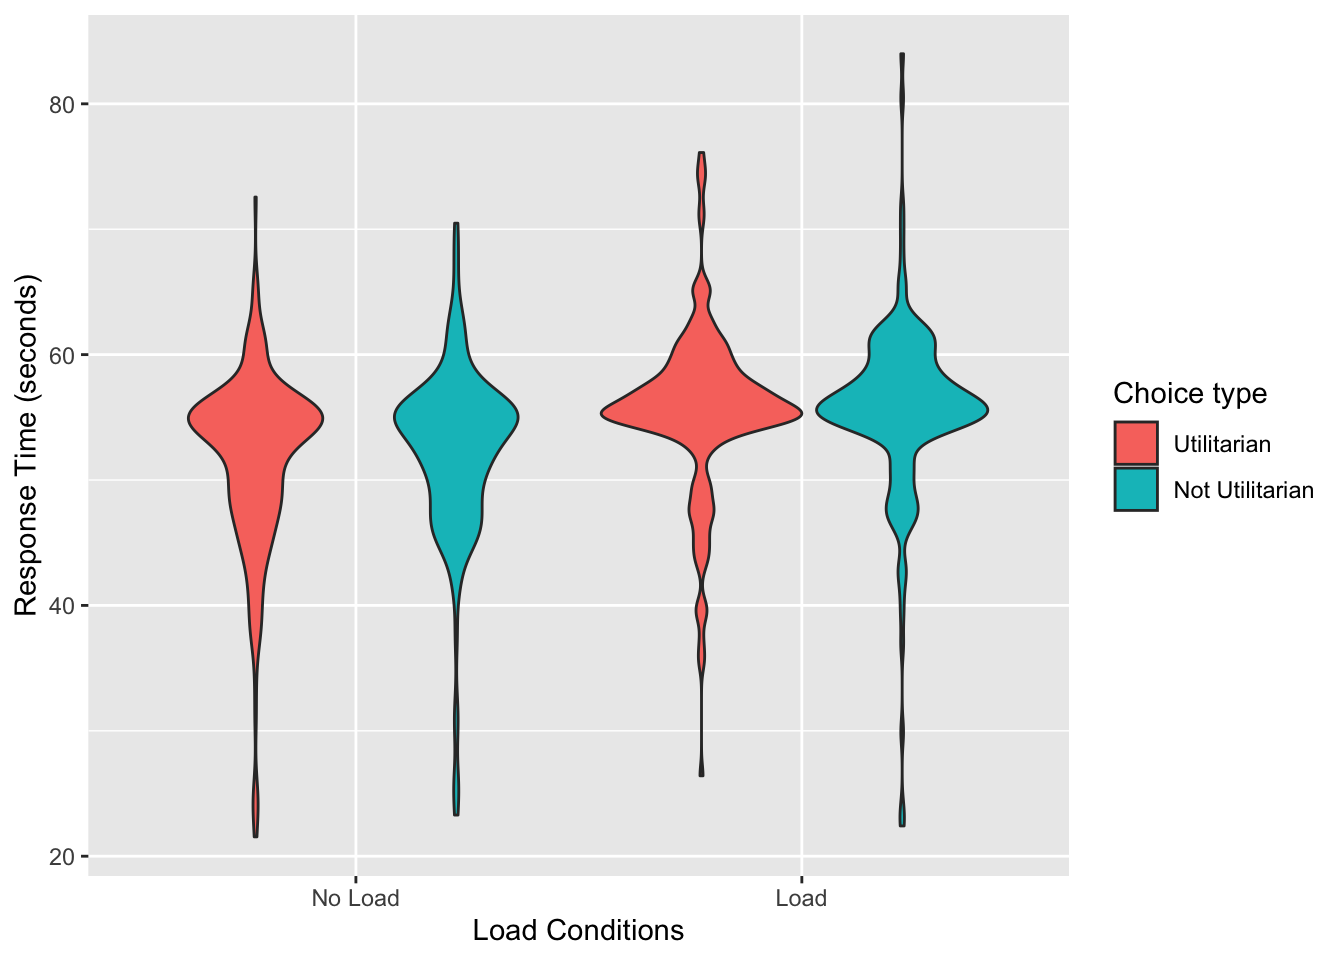
\includegraphics{Reproducibility-Report-Folsom-1222_files/figure-latex/unnamed-chunk-1-1.pdf}

\hypertarget{key-analysis}{%
\subsubsection{Key analysis}\label{key-analysis}}

\begin{Shaded}
\begin{Highlighting}[]
\CommentTok{\#modeling choice}
\NormalTok{m1}\OtherTok{\textless{}{-}} \FunctionTok{lmer}\NormalTok{(rtnum }\SpecialCharTok{\textasciitilde{}}\NormalTok{choicenum }\SpecialCharTok{+}\NormalTok{(}\DecValTok{1}\SpecialCharTok{|}\NormalTok{prolific\_id),}
          \AttributeTok{data =}\NormalTok{ df.datalongtrim)}
\FunctionTok{report}\NormalTok{(m1) }
\end{Highlighting}
\end{Shaded}

\begin{verbatim}
We fitted a linear mixed model (estimated using REML and nloptwrap optimizer) to predict rtnum with choicenum (formula: rtnum ~ choicenum). The model included prolific_id as random effect (formula: ~1 | prolific_id). The model's total explanatory power is substantial (conditional R2 = 0.49) and the part related to the fixed effects alone (marginal R2) is of 2.52e-03. The model's intercept, corresponding to choicenum = 1, is at 53.16 (95% CI [51.84, 54.48], t(791) = 79.11, p < .001). Within this model:

  - The effect of choicenum [2] is statistically non-significant and positive (beta = 0.76, 95% CI [-0.10, 1.61], t(791) = 1.73, p = 0.083; Std. beta = 0.11, 95% CI [-0.01, 0.23])

Standardized parameters were obtained by fitting the model on a standardized version of the dataset. 95% Confidence Intervals (CIs) and p-values were computed using 
\end{verbatim}

\begin{Shaded}
\begin{Highlighting}[]
\FunctionTok{summary}\NormalTok{(m1)}
\end{Highlighting}
\end{Shaded}

\begin{verbatim}
Linear mixed model fit by REML. t-tests use Satterthwaite's method [
lmerModLmerTest]
Formula: rtnum ~ choicenum + (1 | prolific_id)
   Data: df.datalongtrim

REML criterion at convergence: 5083.2

Scaled residuals: 
    Min      1Q  Median      3Q     Max 
-4.4981 -0.4197  0.0793  0.4745  4.6719 

Random effects:
 Groups      Name        Variance Std.Dev.
 prolific_id (Intercept) 27.32    5.227   
 Residual                28.19    5.309   
Number of obs: 795, groups:  prolific_id, 72

Fixed effects:
            Estimate Std. Error       df t value Pr(>|t|)    
(Intercept)  53.1577     0.6719  78.8768  79.111   <2e-16 ***
choicenum2    0.7566     0.4364 758.1595   1.734   0.0834 .  
---
Signif. codes:  0 '***' 0.001 '**' 0.01 '*' 0.05 '.' 0.1 ' ' 1

Correlation of Fixed Effects:
           (Intr)
choicenum2 -0.278
\end{verbatim}

\begin{Shaded}
\begin{Highlighting}[]
\CommentTok{\#modeling load }
\NormalTok{m2 }\OtherTok{\textless{}{-}} \FunctionTok{lmer}\NormalTok{(rtnum }\SpecialCharTok{\textasciitilde{}}\NormalTok{load }\SpecialCharTok{+}\NormalTok{(}\DecValTok{1}\SpecialCharTok{|}\NormalTok{prolific\_id),}
           \AttributeTok{data =}\NormalTok{ df.datalongtrim)}
\FunctionTok{report}\NormalTok{(m2)}
\end{Highlighting}
\end{Shaded}

\begin{verbatim}
We fitted a linear mixed model (estimated using REML and nloptwrap optimizer) to predict rtnum with load (formula: rtnum ~ load). The model included prolific_id as random effect (formula: ~1 | prolific_id). The model's total explanatory power is substantial (conditional R2 = 0.55) and the part related to the fixed effects alone (marginal R2) is of 0.06. The model's intercept, corresponding to load = l1, is at 51.69 (95% CI [50.39, 52.99], t(791) = 77.99, p < .001). Within this model:

  - The effect of load [l2] is statistically significant and positive (beta = 3.59, 95% CI [2.89, 4.29], t(791) = 10.10, p < .001; Std. beta = 0.50, 95% CI [0.41, 0.60])

Standardized parameters were obtained by fitting the model on a standardized version of the dataset. 95% Confidence Intervals (CIs) and p-values were computed using 
\end{verbatim}

\begin{Shaded}
\begin{Highlighting}[]
\FunctionTok{summary}\NormalTok{(m2)}
\end{Highlighting}
\end{Shaded}

\begin{verbatim}
Linear mixed model fit by REML. t-tests use Satterthwaite's method [
lmerModLmerTest]
Formula: rtnum ~ load + (1 | prolific_id)
   Data: df.datalongtrim

REML criterion at convergence: 4990.9

Scaled residuals: 
    Min      1Q  Median      3Q     Max 
-5.0549 -0.3849  0.0635  0.4751  5.1037 

Random effects:
 Groups      Name        Variance Std.Dev.
 prolific_id (Intercept) 27.00    5.196   
 Residual                24.85    4.985   
Number of obs: 795, groups:  prolific_id, 72

Fixed effects:
            Estimate Std. Error       df t value Pr(>|t|)    
(Intercept)  51.6882     0.6627  78.9740   77.99   <2e-16 ***
loadl2        3.5910     0.3556 721.2864   10.10   <2e-16 ***
---
Signif. codes:  0 '***' 0.001 '**' 0.01 '*' 0.05 '.' 0.1 ' ' 1

Correlation of Fixed Effects:
       (Intr)
loadl2 -0.267
\end{verbatim}

\begin{Shaded}
\begin{Highlighting}[]
\CommentTok{\#model the load*choice and rt}
\NormalTok{m3 }\OtherTok{\textless{}{-}} \FunctionTok{lmer}\NormalTok{(rtnum }\SpecialCharTok{\textasciitilde{}}\NormalTok{load }\SpecialCharTok{*}\NormalTok{choicenum }\SpecialCharTok{+}\NormalTok{(}\DecValTok{1}\SpecialCharTok{|}\NormalTok{prolific\_id),}
           \AttributeTok{data =}\NormalTok{ df.datalongtrim)}
\FunctionTok{report}\NormalTok{(m3)}
\end{Highlighting}
\end{Shaded}

\begin{verbatim}
We fitted a linear mixed model (estimated using REML and nloptwrap optimizer) to predict rtnum with load and choicenum (formula: rtnum ~ load * choicenum). The model included prolific_id as random effect (formula: ~1 | prolific_id). The model's total explanatory power is substantial (conditional R2 = 0.55) and the part related to the fixed effects alone (marginal R2) is of 0.06. The model's intercept, corresponding to load = l1 and choicenum = 1, is at 51.38 (95% CI [50.01, 52.75], t(789) = 73.67, p < .001). Within this model:

  - The effect of load [l2] is statistically significant and positive (beta = 4.01, 95% CI [3.07, 4.95], t(789) = 8.41, p < .001; Std. beta = 0.56, 95% CI [0.43, 0.70])
  - The effect of choicenum [2] is statistically non-significant and positive (beta = 0.82, 95% CI [-0.28, 1.92], t(789) = 1.46, p = 0.144; Std. beta = 0.12, 95% CI [-0.04, 0.27])
  - The interaction effect of choicenum [2] on load [l2] is statistically non-significant and negative (beta = -1.05, 95% CI [-2.50, 0.40], t(789) = -1.42, p = 0.155; Std. beta = -0.15, 95% CI [-0.35, 0.06])

Standardized parameters were obtained by fitting the model on a standardized version of the dataset. 95% Confidence Intervals (CIs) and p-values were computed using 
\end{verbatim}

\begin{Shaded}
\begin{Highlighting}[]
\FunctionTok{summary}\NormalTok{(m3)}
\end{Highlighting}
\end{Shaded}

\begin{verbatim}
Linear mixed model fit by REML. t-tests use Satterthwaite's method [
lmerModLmerTest]
Formula: rtnum ~ load * choicenum + (1 | prolific_id)
   Data: df.datalongtrim

REML criterion at convergence: 4987.2

Scaled residuals: 
    Min      1Q  Median      3Q     Max 
-5.0437 -0.3848  0.0564  0.4657  5.0542 

Random effects:
 Groups      Name        Variance Std.Dev.
 prolific_id (Intercept) 27.14    5.210   
 Residual                24.82    4.982   
Number of obs: 795, groups:  prolific_id, 72

Fixed effects:
                  Estimate Std. Error       df t value Pr(>|t|)    
(Intercept)        51.3770     0.6974  95.3172  73.673   <2e-16 ***
loadl2              4.0102     0.4766 721.3052   8.415   <2e-16 ***
choicenum2          0.8204     0.5616 741.4926   1.461    0.144    
loadl2:choicenum2  -1.0490     0.7374 724.0550  -1.422    0.155    
---
Signif. codes:  0 '***' 0.001 '**' 0.01 '*' 0.05 '.' 0.1 ' ' 1

Correlation of Fixed Effects:
            (Intr) loadl2 chcnm2
loadl2      -0.307              
choicenum2  -0.305  0.383       
ldl2:chcnm2  0.207 -0.660 -0.678
\end{verbatim}

\begin{Shaded}
\begin{Highlighting}[]
\CommentTok{\#looking at model comparisons}
\FunctionTok{anova}\NormalTok{(m2, m3)}
\end{Highlighting}
\end{Shaded}

\begin{verbatim}
refitting model(s) with ML (instead of REML)
\end{verbatim}

\begin{verbatim}
Data: df.datalongtrim
Models:
m2: rtnum ~ load + (1 | prolific_id)
m3: rtnum ~ load * choicenum + (1 | prolific_id)
   npar    AIC    BIC  logLik deviance  Chisq Df Pr(>Chisq)
m2    4 4999.7 5018.4 -2495.8   4991.7                     
m3    6 5001.2 5029.2 -2494.6   4989.2 2.4809  2     0.2893
\end{verbatim}

\begin{Shaded}
\begin{Highlighting}[]
\FunctionTok{anova}\NormalTok{(m1, m2)}
\end{Highlighting}
\end{Shaded}

\begin{verbatim}
refitting model(s) with ML (instead of REML)
\end{verbatim}

\begin{verbatim}
Data: df.datalongtrim
Models:
m1: rtnum ~ choicenum + (1 | prolific_id)
m2: rtnum ~ load + (1 | prolific_id)
   npar    AIC    BIC  logLik deviance  Chisq Df Pr(>Chisq)
m1    4 5092.3 5111.1 -2542.2   5084.3                     
m2    4 4999.7 5018.4 -2495.8   4991.7 92.693  0           
\end{verbatim}

\begin{Shaded}
\begin{Highlighting}[]
\FunctionTok{anova}\NormalTok{(m1, m3)}
\end{Highlighting}
\end{Shaded}

\begin{verbatim}
refitting model(s) with ML (instead of REML)
\end{verbatim}

\begin{verbatim}
Data: df.datalongtrim
Models:
m1: rtnum ~ choicenum + (1 | prolific_id)
m3: rtnum ~ load * choicenum + (1 | prolific_id)
   npar    AIC    BIC  logLik deviance  Chisq Df Pr(>Chisq)    
m1    4 5092.3 5111.1 -2542.2   5084.3                         
m3    6 5001.2 5029.2 -2494.6   4989.2 95.174  2  < 2.2e-16 ***
---
Signif. codes:  0 '***' 0.001 '**' 0.01 '*' 0.05 '.' 0.1 ' ' 1
\end{verbatim}

\begin{Shaded}
\begin{Highlighting}[]
\CommentTok{\#save model outputs to make a figure}
\NormalTok{means }\OtherTok{\textless{}{-}} \FunctionTok{estimate\_means}\NormalTok{(m3)}
\end{Highlighting}
\end{Shaded}

\begin{verbatim}
We selected `at = c("load", "choicenum")`.
\end{verbatim}

\begin{Shaded}
\begin{Highlighting}[]
\FunctionTok{as.factor}\NormalTok{(means}\SpecialCharTok{$}\NormalTok{load) }\CommentTok{\#this will make the graphing easier}
\end{Highlighting}
\end{Shaded}

\begin{verbatim}
[1] l1 l2 l1 l2
Levels: l1 l2
\end{verbatim}

\begin{Shaded}
\begin{Highlighting}[]
\NormalTok{means }\SpecialCharTok{\%\textgreater{}\%} 
  \FunctionTok{ggplot}\NormalTok{(}\AttributeTok{mapping =} \FunctionTok{aes}\NormalTok{(}\AttributeTok{x =}\NormalTok{ load,}
                       \AttributeTok{y =}\NormalTok{ Mean,}
                       \AttributeTok{group =}\NormalTok{ choicenum,}
                       \AttributeTok{color =}\NormalTok{ choicenum}
\NormalTok{                        ))}\SpecialCharTok{+}
  \FunctionTok{geom\_line}\NormalTok{(}\AttributeTok{size =} \FloatTok{1.5}\NormalTok{)}\SpecialCharTok{+}
  \FunctionTok{geom\_errorbar}\NormalTok{(}\FunctionTok{aes}\NormalTok{(}\AttributeTok{ymin=}\NormalTok{CI\_low, }\AttributeTok{ymax=}\NormalTok{CI\_high), }\AttributeTok{width=}\NormalTok{.}\DecValTok{05}\NormalTok{, }\AttributeTok{size =} \FloatTok{0.6}\NormalTok{)}\SpecialCharTok{+}
  \FunctionTok{geom\_point}\NormalTok{()}\SpecialCharTok{+}
  \FunctionTok{labs}\NormalTok{(}\AttributeTok{title =} \StringTok{"Effect of Load and Moral Choice on RT"}\NormalTok{,}
       \AttributeTok{x =} \StringTok{"Load Conditions"}\NormalTok{,}
       \AttributeTok{y =} \StringTok{"Response Time Means (seconds)"}\NormalTok{)}\SpecialCharTok{+}
  \FunctionTok{scale\_x\_discrete}\NormalTok{(}\AttributeTok{labels=}\FunctionTok{c}\NormalTok{(}\StringTok{"l1"} \OtherTok{=} \StringTok{"No Load"}\NormalTok{,}
                            \StringTok{"l2"} \OtherTok{=} \StringTok{"Load"}\NormalTok{))}\SpecialCharTok{+}
  \FunctionTok{scale\_colour\_grey}\NormalTok{(}\AttributeTok{name=}\StringTok{"Choice type"}\NormalTok{,}
                  \AttributeTok{labels=}\FunctionTok{c}\NormalTok{(}\StringTok{"1"} \OtherTok{=} \StringTok{"Utilitarian"}\NormalTok{,}
                           \StringTok{"2"} \OtherTok{=} \StringTok{"Not Utilitarian"}\NormalTok{),}
                  \AttributeTok{start =} \FloatTok{0.3}\NormalTok{,}
                  \AttributeTok{end =} \FloatTok{0.7}\NormalTok{)}
\end{Highlighting}
\end{Shaded}

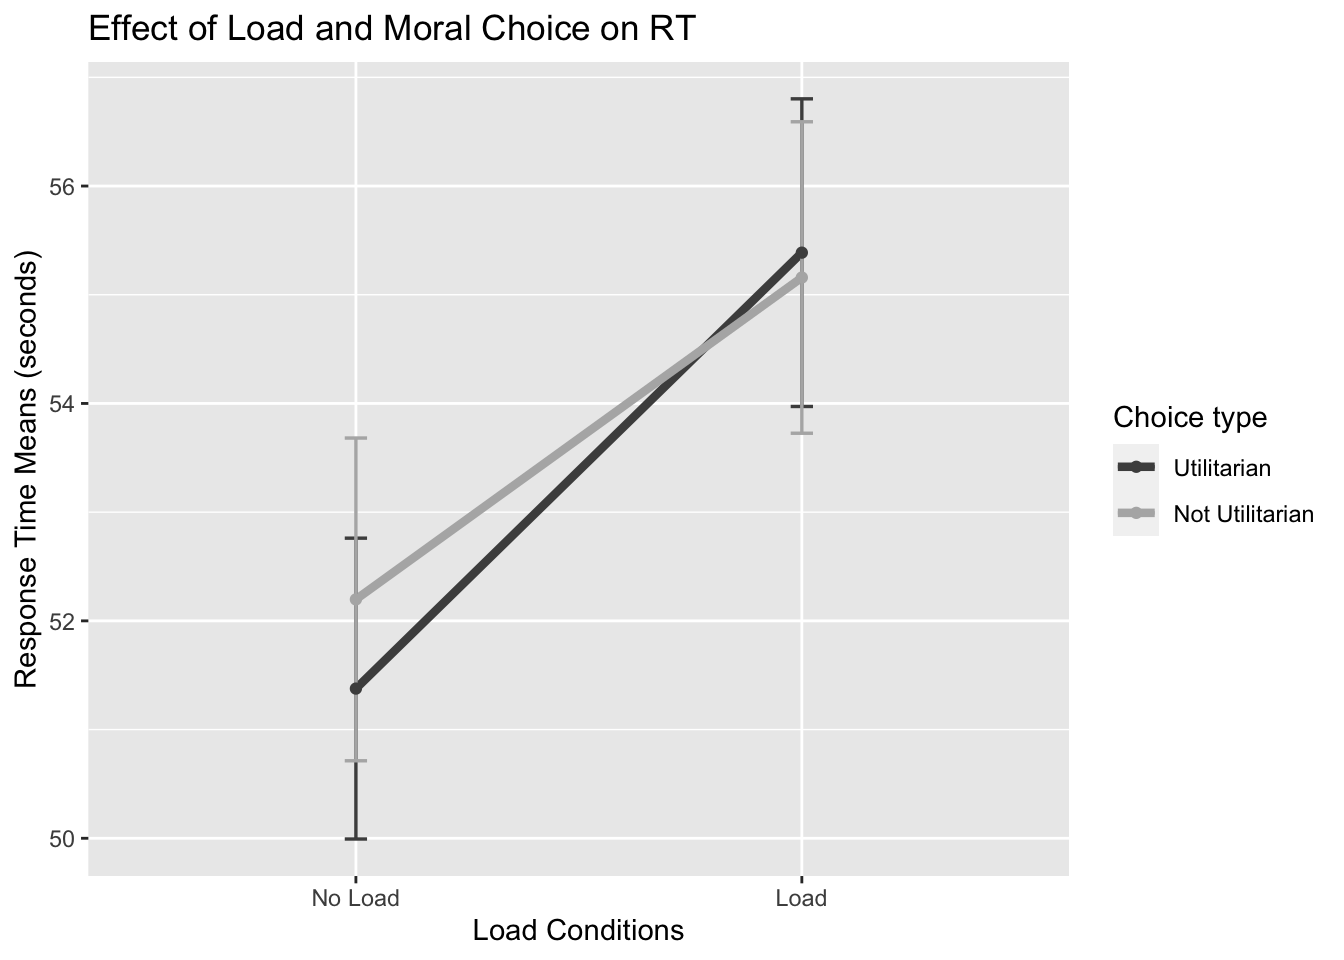
\includegraphics{Reproducibility-Report-Folsom-1222_files/figure-latex/model time-1.pdf}
The analyses as specified in the analysis plan.

\begin{Shaded}
\begin{Highlighting}[]
\FunctionTok{include\_graphics}\NormalTok{(}\StringTok{"Figures/Greene\_Fig1.png"}\NormalTok{)}
\end{Highlighting}
\end{Shaded}

\begin{figure}
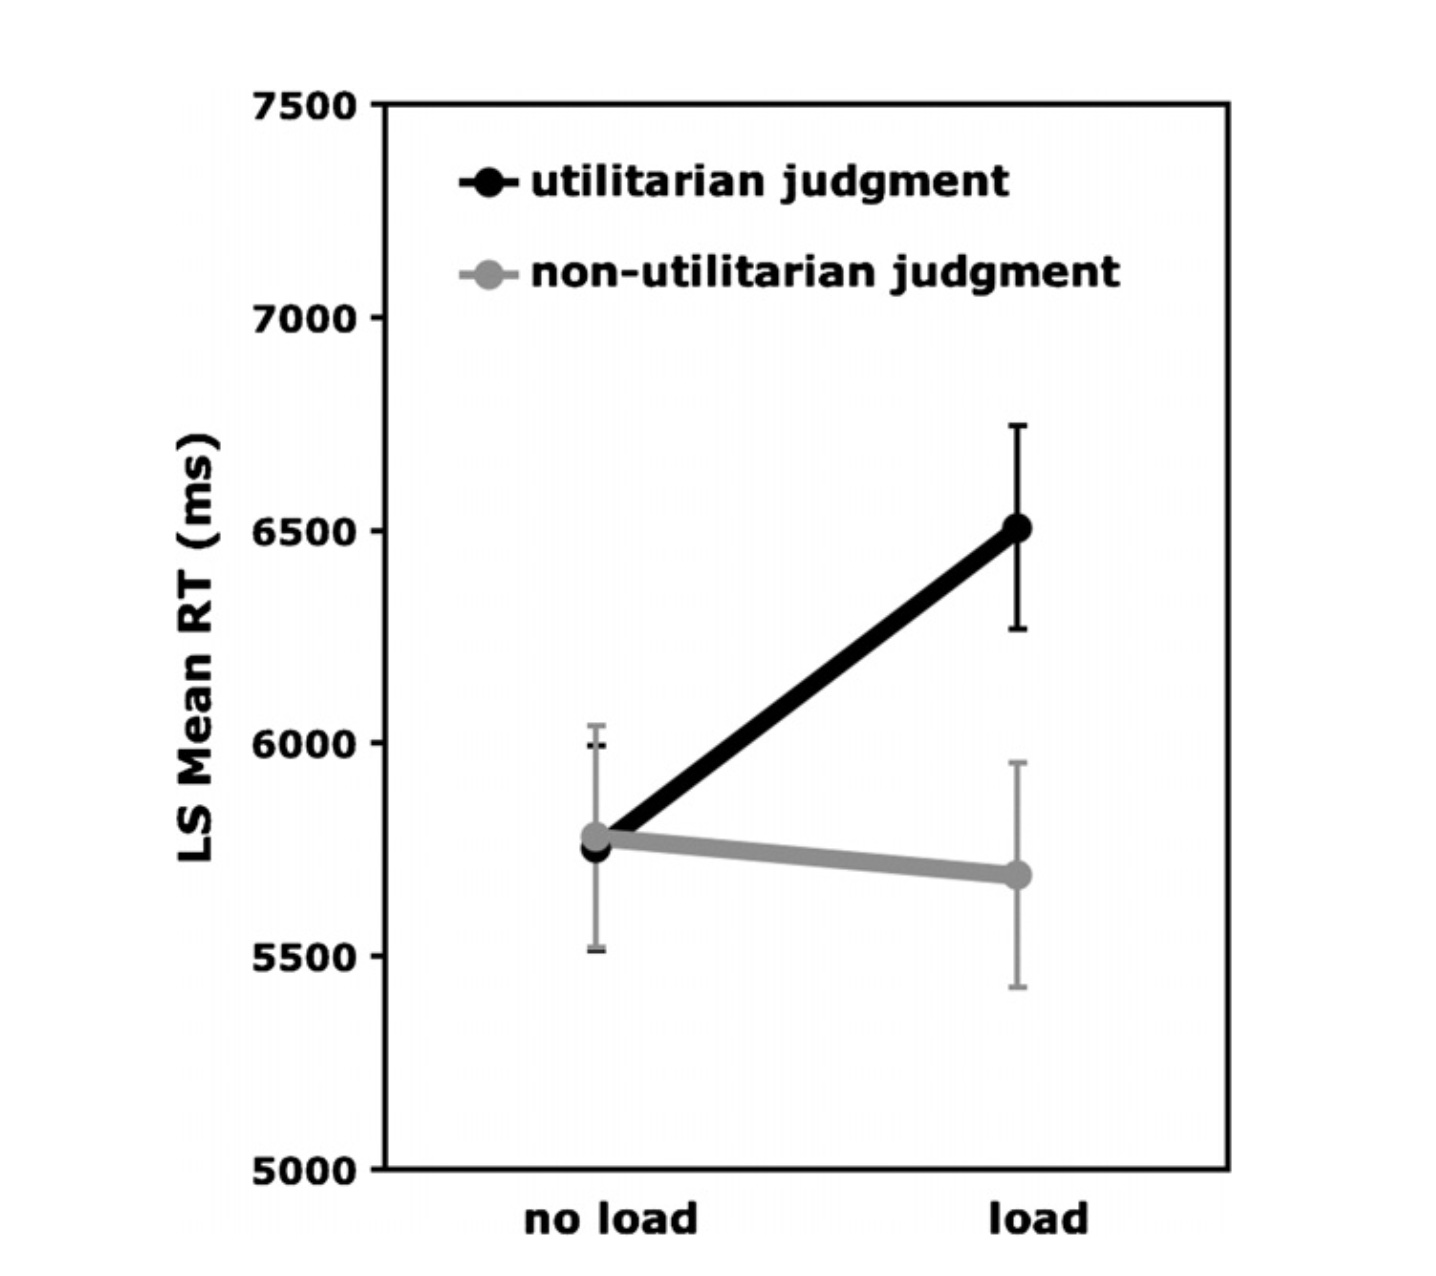
\includegraphics[width=0.8\linewidth]{Figures/Greene_Fig1} \caption{Greene}\label{fig:unnamed-chunk-2}
\end{figure}

\hypertarget{discussion}{%
\subsection{Discussion}\label{discussion}}

\hypertarget{summary-of-reproduction-attempt}{%
\subsubsection{Summary of Reproduction
Attempt}\label{summary-of-reproduction-attempt}}

Open the discussion section with a paragraph summarizing the primary
result from the key analysis and assess whether you successfully
reproduced it, partially reproduced it, or failed to reproduce it.

Unfortunately we were unsuccessful in reproducing the original paper's
findings.

\hypertarget{commentary}{%
\subsubsection{Commentary}\label{commentary}}

Add open-ended commentary (if any) reflecting (a) insights from
follow-up exploratory analysis of the dataset, (b) assessment of the
meaning of the successful or unsuccessful reproducibility attempt -
e.g., for a failure to reproduce the original findings, are the
differences between original and present analyses ones that definitely,
plausibly, or are unlikely to have been moderators of the result, and
(c) discussion of any objections or challenges raised by the current and
original authors about the reproducibility attempt (if you contacted
them). None of these need to be long.

\end{document}
